%% LyX 2.1.4 created this file.  For more info, see http://www.lyx.org/.
%% Do not edit unless you really know what you are doing.
\documentclass[english]{article}
\usepackage[T1]{fontenc}
\usepackage[latin9]{inputenc}
\usepackage{geometry}
\geometry{verbose,tmargin=2cm,bmargin=3cm,lmargin=1.5cm,rmargin=1.5cm}
\usepackage{float}
\usepackage{mathtools}
\usepackage{amsmath}
\usepackage{amssymb}
\usepackage{graphicx}

\makeatletter

%%%%%%%%%%%%%%%%%%%%%%%%%%%%%% LyX specific LaTeX commands.
%% Because html converters don't know tabularnewline
\providecommand{\tabularnewline}{\\}
\floatstyle{ruled}
\newfloat{algorithm}{tbp}{loa}
\providecommand{\algorithmname}{Algorithm}
\floatname{algorithm}{\protect\algorithmname}

%%%%%%%%%%%%%%%%%%%%%%%%%%%%%% User specified LaTeX commands.
\usepackage{tikz}
\usepackage{babel}
\renewcommand{\labelitemi}{$\diamond$}
\newcommand{\T}{\rule{0pt}{2.6ex}}       % Top strut
\newcommand{\B}{\rule[-1.2ex]{0pt}{0pt}} % Bottom strut
\usepackage{algorithm,algpseudocode}

\makeatother

\usepackage{babel}
\begin{document}

\title{COMP8620: MC-AIXI-CTW\\
Group 3}


\author{Jarryd Martin, John Aslanides, Yadunandan Sannappa,\\
 Nrupendra Rao, Cheng Yu, Ryk Budzynski}


\date{October 2015}

\maketitle
We outline an implementation of Veness et al.'s Monte Carlo AIXI approximation\cite{veness-11}
(MC-AIXI-CTW), and report our simulation results on a number of toy
domains.


\section{Introduction}

Recall that the AIXI agent is defined by its actions, which for each
cycle $k$ are given by 
\[
a_{k}^{\text{AIXI}}=\arg\max_{a_{k}}\sum_{o_{k}r_{k}}\cdots\max_{a_{m}}\sum_{o_{m}r_{m}}\left[r_{k}+\dots+r_{m}\right]\xi\left(o_{1}r_{1}\dots o_{m}r_{m}|a_{1}\dots a_{m}\right),
\]


where the $o_{n}$ and $r_{n}$ are the observation and reward provided
by the environment at cycle $n$, and $\xi$ is a Bayesian mixture
model for the environment. 

Following Veness et al., we approximate $a_{k}^{\text{AIXI}}$ using
Monte Carlo tree search (upper confidence bound) to approximate the
expectimax, and we compute a mixture over variable-order Markov models
using the context-tree weighting algorithm. 

We present a lightweight C++ implementation of MC-AIXI-CTW, along
with implementations of a number of simple games: $\textsc{Pacman},\ $
$\textsc{Tic-Tac-Toe}$, $\textsc{Biased Rock-Paper-Scissor}$, $\textsc{Extended-Tiger}$,
and $\textsc{Cheesemaze}$.


\section{User Manual}

To build from source, run ${\tt g++\ *.cpp\ *.hpp\ -o\ aixi}$ \textbf{TODO
check}

To run, invoke ${\tt ./aixi\ envname}$. 


\section{MC-AIXI-CTW Implementation}


\subsection{Main loop}

For each agent-environment interaction cycle, we run the following
for each experiment:

\begin{algorithm}
\begin{algorithmic}[1]
\renewcommand{\algorithmicrequire}{\textbf{Inputs:}}
\renewcommand{\algorithmicensure}{\textbf{Outputs:}}
\While{$cycle < max\_cycles$}
\While{environment is not finished}
\State{generate $(o,r)$ from environment}
\State{update agent model with $(o,r)$}
\If{explore}
\State{$a \leftarrow randomAction()$}
\Else
\State{$a \leftarrow MCTS()$}
\Comment{Monte Carlo Tree Search}
\EndIf
\State{perform action $a$}
\State{update agent history with $a$}
\State{$cycle++$}
\EndWhile
\State{reset environment}
\EndWhile
\end{algorithmic}

\caption{Main loop.}


\end{algorithm}


The $MCTS$ algorithm follows as in Algorithms 1-4 in Veness et al.,
and is found in ${\tt search.cpp}$. Model updates are handled in
methods in ${\tt agent.cpp}$, which interfaces with the context tree
defined in ${\tt predict.cpp}$.


\subsection{Monte Carlo Tree Search (MCTS) Algorithm}


\subsubsection{High level description}

Since the environment is only partially observable, we have no explicit
notion of state; instead, we only have a history of actions and percepts
$h=\left(a_{1}o_{1}r_{1}\dots a_{n}o_{n}r_{n}\right)$. For the purposes
of choosing the optimal action, we treat each possible (hypothetical)
history as a node in the search tree, with the root being the tip
of the current (realised) history. Each node is labelled by its history.
The expected value of each node in the search tree is equal to the
expected total (non-discounted) reward that would be accumulated from
that node, where the expectation is under the agent's current policy
and the agent's current model for the behavior of the environment. 

Thus, for each node we keep a value estimate $\hat{V}$, and a count
of the number of times $T$ that node has been visited in search.
This is used to determine how we explore the search space using the
UCB algorithm, which, for each decision node picks (assuming $T\left(ha\right)>0$
for all actions)
\[
a_{\text{UCB}}=\arg\max_{a\in\mathcal{A}}\left\{ \frac{1}{m\left(\beta-\alpha\right)}\hat{V}\left(ha\right)+C\sqrt{\frac{\log T\left(h\right)}{T\left(ha\right)}}\right\} ,
\]


where $\mathcal{A}$ is the set of all permissible actions, $m$ is
the search horizon, $\beta-\alpha$ is the difference between the
minimal and maximal instantaneous reward, and $C$ is a parameter
controlling the propensity of the agent to explore less frequently-seen
histories. 

Note that the expectimax is a stochastic, partially observable game
between the agent and its environment. In the following, call nodes
corresponding to agent moves `decision nodes', and nodes corresponding
to Nature's moves `chance nodes'.


\subsubsection{Class structure}

To represent our search nodes, we define a base ${\tt SearchNode}$
class, from which ChanceNode and DecisionNode inherit. ChanceNode
and DecisionNode each have a ${\tt sample}$ method defined on them;
each of these methods is mutually recursive. For a given node $n$,
we keep its children in a dictionary keyed on the action or (observation,reward)
used to generate each child.


\subsubsection{Code snippets}


\subsubsection{Efficiency/performance}


\subsection{Context Tree Weighting (CTW)}


\subsubsection{High level description of algorithm}


\subsubsection{Class structure}


\subsubsection{Code snippets}


\subsubsection{Efficiency/performance}


\subsection{Environments}


\subsubsection{Cheesemaze}


\subsubsection{Extended Tiger}


\subsubsection{Biased Rock-Paper-Scissor}


\subsubsection{Tic-Tac-Toe}


\subsubsection{Pacman}


\section{Simulation Results}


\subsection{Cheesemaze}
\begin{itemize}
\item Experimental setup ... \\
 Any simulation provided should include detailed description of experimental
setup; selected parameters of algorithms and examples; and concise
interpretations of obtained simulation results. \\



\begin{tabular}{|l|l|l|}
\hline 
Environment  & MCTS  & CTW \tabularnewline
\hline 
1  & $m=100$  & $\text{ct-depth}=96$ \tabularnewline
\hline 
 & $C=\sqrt{2}$  & \tabularnewline
\hline 
\end{tabular}

\item Plots ... \\
 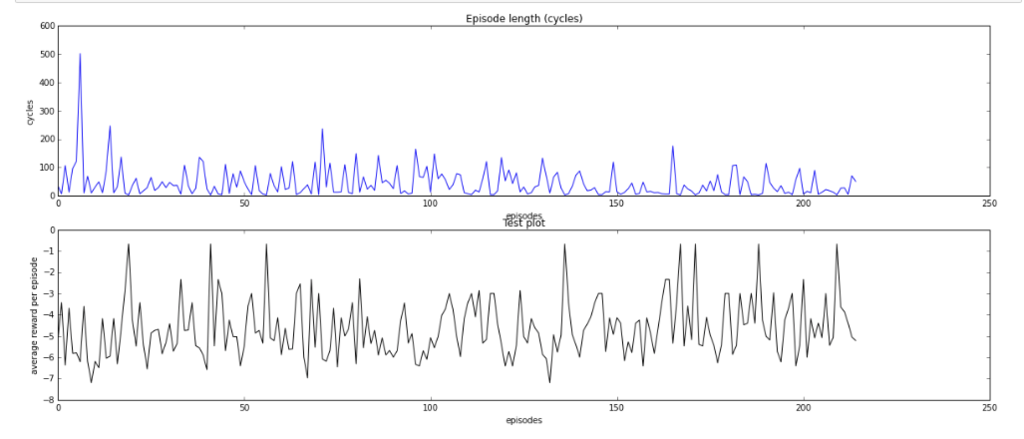
\includegraphics[scale=0.4]{cheesemaze_01} 
\item Interpretation of Results 
\end{itemize}

\subsection{Extended Tiger}

Experimental setup ... \\
 Plots ... 


\subsection{Biased Rock-Paper-Scissor}

Experimental setup ... \\
 Plots ... 


\subsection{Tic-Tac-Toe}

Experimental setup ... \\
 Plots ... 


\subsection{Pacman}

Experimental setup ... \\
 Plots ... 


\section{Cross Domain Simulation Results}
\begin{itemize}
\item Cheesemaze and Extended Tiger
\item Cross domain simulation on more difficult environments... 
\item Separate CTW for Obs and Rews...
\end{itemize}

\section{Discussion and Conclusions}


\section*{Appendix}

\appendix

\section{Files}

The report archive should contain the following: 
\begin{verbatim}

MC-AIXI-CTW-Grp3.zip
    \report
        report.pdf // this report
        report.tex
        cheesemaze_01.png // results plots
        extended_tiger_01.png
        biased_rock_paper_scissor_01.png
        tic_tac_toe_01.png
        pacman_01.png
    \src
        main.hpp
        main.cpp
        environment.hpp
        environment.cpp
        agent.hpp
        agent.cpp
        search.hpp
        search.cpp
        predict.hpp
        predict.cpp
        util.hpp
        util.cpp
        README.md
        cheesemaze.conf // environment configuration files
        rockpaper.conf
        tictactoe.conf
        coinflip.conf
        tiger.conf
\end{verbatim}
\bibliographystyle{unsrt}
\bibliography{report}

\end{document}
